\section{Output}

Intro text required




\subsection{HDMI}

HDMI is a two-way communication protocol and supports many different formats/frequencies/specs. Many monitors/recorders only support a subset of these formats and expect signals to conform to certain values. These values are not documented publicly so we are currently in the process of debugging device compatibility one by one. The good thing is that it's a pure software thing and we can add support and test compatibility with additional devices as time progresses.\\

In general we discovered that monitors are more flexible when it comes to HDMI (TMDS) freqencies as they just "tune" into (sync to) the provided clock/data rate. Recorders expect signals to be in a much stricter/narrower range and will not work (show "no signal") if there is a minor deviation. 

Watch this 33C3 talk by Tim Ansell about \href{https://media.ccc.de/v/33c3-8057-dissecting_hdmi}{Dissecting HDMI} to get insight into how HDMI works.




\subsubsection{External HDMI Recording}

Settings for VSync, HSync, etc. inside the AXIOM Beta can be found in: 

\consoleCommand{/root/gen\_init.sh}

For example the Atomos SHOGUN was found to work with these HDMI parameters:  

\begin{lstlisting}[breaklines=true, breakatwhitespace=true]
scn\_reg  0 2200             # total\_w
scn\_reg  1 1125             # total\_h
scn\_reg  2   60             # total\_f

scn\_reg  4  262             # hdisp\_s
scn\_reg  5 2182             # hdisp\_e
scn\_reg  6   45             # vdisp\_s
scn\_reg  7 1125             # vdisp\_e

scn\_reg  8    0             # hsync\_s
scn\_reg  9 2100             # hsync\_e
scn\_reg 10    4             # vsync\_s
scn\_reg 11    9             # vsync\_e

scn\_reg 32  252             # pream\_s
scn\_reg 33  260             # guard\_s
scn\_reg 34  294             # terc4\_e
scn\_reg 35  296             # guard\_e
\end{lstlisting}

Currently it is not possible to alter TMDS and Clock frequencies from the userspace (requires new FPGA bitstream).\\

For the firmware there are two modes available, the 30Hz and 60Hz variant. You can switch between them quite easily.\\

cmv\_hdmi3.bit is the FPGA bitstream loaded for the HDMI interface. We use symlinks to switch this file easily.\\

Before doing this, don't forget to check if the files (cmv\_hdmi3\_60.bit or cmv\_hdmi3\_30.bit) really exist in the /root folder.\\

The output is always in 8bpc RGB color space without subsampling (4:4:4). Not all capture devices can manage this.\\

Other modes like YCrCb, etc. are currently not supported.\\ 




\paragraph{Devices Confirmed Working}

Atomos Shogun - AXIOM Beta supports up to 1080p60 
Atomos Ninja - AXIOM Beta supports up to 1080p30
Blackmagic Video Assist and Video Assist 4K - AXIOM Beta supports up to 1080p60\\

\textbf{Blackmagic Video Assist and Video Assist 4K}

\begin{center}
	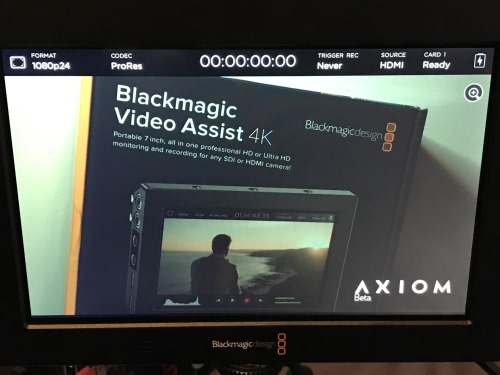
\includegraphics[height=8cm]{images/AxiomBetaBMVA4K}\\
\end{center}

Changes for Blackmagic Video Assist and Video Assist 4K, tested on firmware 2.3.1:\\

\textbf{edit setup.sh}\\

Add: 

\consoleCommand{./gen\_init.sh 1080p60BMVA}

comment out any other ./gen\_init.sh entries. 

\textbf{edit gen\_init.sh}

\consoleCommand{./gen\_init.sh 1080p60BMVA}

\textbf{edit gen\_init.sh}

Replace:

\consoleCommand{SHOGUN)}

With:

\consoleCommand{SHOGUN|1080p60BMVA|1080p30BMVA)}

Add the section below:

\consoleCommand{  
	1080p50BMVA|1080p25BMVA)^^J
	scn\_reg  0 2640	# total\_w^^J
	scn\_reg  1 1125    # total\_h^^J
	scn\_reg  2   60    # total\_f^^J
	^^J
	scn\_reg  4  262    # hdisp\_s^^J
	scn\_reg  5 2182    # hdisp\_e^^J
	scn\_reg  6   45    # vdisp\_s^^J
	scn\_reg  7 1125    # vdisp\_e^^J
	^^J
	scn\_reg  8    0    # hsync\_s^^J
	scn\_reg  9 2100    # hsync\_e^^J
	scn\_reg 10    4    # vsync\_s^^J
	scn\_reg 11    9    # vsync\_e^^J
	^^J
	scn\_reg 32  252	# pream\_s^^J
	scn\_reg 33  260    # guard\_s^^J
	scn\_reg 34  294    # terc4\_e^^J
	scn\_reg 35  296    # guard\_e^^J
	;;
	^^J
	^^J
	1080p24BMVA)^^J
	scn\_reg  0 2750    # total\_w^^J
	scn\_reg  1 1125    # total\_h^^J
	scn\_reg  2   60    # total\_f^^J
	^^J
	scn\_reg  4  262    # hdisp\_s^^J
	scn\_reg  5 2182    # hdisp\_e^^J
	scn\_reg  6   45    # vdisp\_s^^J
	scn\_reg  7 1125    # vdisp\_e^^J
	^^J
	scn\_reg  8    0    # hsync\_s^^J
	scn\_reg  9 2100    # hsync\_e^^J
	scn\_reg 10    4    # vsync\_s^^J
	scn\_reg 11    9    # vsync\_e^^J
	^^J
	scn\_reg 32  252    # pream\_s^^J
	scn\_reg 33  260    # guard\_s^^J
	scn\_reg 34  294    # terc4\_e^^J
	scn\_reg 35  296    # guard\_e^^J
	;;
}




\subsubsection{Experimental UHD Raw Recording}

\textbf{Note:} This experimental raw mode works only in 1080p60 (A+B Frames) and is only tested with the Atomos Shogun currently. \\

To measure the required compensations with a different recorder see \textbf{Raw processing recorder benchmarking}\\

This mode requires darkframes which are created in the course of a camera Factory Calibration. Early Betas are not calibrated yet - this step needs to be completed by the user. See \textbf{Factory Calibration}.\\




\paragraph{Enable raw recording mode}\mbox{}\\

Input:

\consoleCommand{\./hdmi\_rectest.sh}

Inside that script the following command is worth noting:\\

Enable experimental raw mode: 

\consoleCommand{scn\_reg 31 0x0A01}

Disable experimental raw mode: 

\consoleCommand{scn\_reg 31 0x0001}

If you get an error report like this: 

\consoleCommand{    Traceback (most recent call last):
	File "rcn\_darkframe\.py", line 17, in <module>
	import png
	ImportError: No module named 'png'}

Make sure the Beta is connected to the Internet via Ethernet and run:     

\consoleCommand{pip install pypng}




\paragraph{Processing}

Postprocessing software to recover the raw information (DNG sequences) is on github in \href{https://github.com/apertus-open-source-cinema/misc-tools-utilities/tree/master/raw-via-hdmi}{RAW via HDMI}

Required packages: ffmpeg build-essentials

Mac requirements for compiling: gcc4.9(via homebrew): 

\consoleCommand{brew install homebrew/versions/gcc49}

Also install ffmpeg\\

To do all the raw processing in one single command (after ffmpeg codec copy processing): 

\consoleCommand{\./hdmi4k INPUT\.MOV - | \./raw2dng --fixrnt --pgm --black=120 frame\%05d\.dng}
	
	
	
	
\subsubsection{Experimental UHD Raw Recording}

\textbf{Note:} This experimental raw mode works only in 1080p60 (A+B Frames) and is only tested with the Atomos Shogun currently. \\

To measure the required compensations with a different recorder see \textbf{Raw processing recorder benchmarking}\\

This mode requires darkframes which are created in the course of a camera Factory Calibration. Early Betas are not calibrated yet - this step needs to be completed by the user. See \textbf{Factory Calibration}.\\




\paragraph{Enable raw recording mode}\mbox{}\\

Input:

\consoleCommand{\./hdmi\_rectest.sh}

Inside that script the following command is worth noting:\\

Enable experimental raw mode: 

\consoleCommand{scn\_reg 31 0x0A01}

Disable experimental raw mode: 

\consoleCommand{scn\_reg 31 0x0001}

If you get an error report like this: 

\consoleCommand{    Traceback (most recent call last):
	File "rcn\_darkframe\.py", line 17, in <module>
	import png
	ImportError: No module named 'png'}

Make sure the Beta is connected to the Internet via Ethernet and run:     

\consoleCommand{pip install pypng}




\subparagraph{Raw processing recorder benchmarking}
	
We can analyze footage recorded by the 3rd party recorder but we would need the following:\\
	
- Make sure your Beta is running in experimental 4k raw mode (1080p60 with A+B frames)\\
- Short HDMI captured clip from the 3rd party recorder\\
- Raw12 still image captured during the HDMI recording\\
	
This kind of script is helpful to execute during HDMI recording: 
	
\consoleCommand{
	# stop HDMI stream:^^J
	fil\_reg 15 0^^J
	^^J
	# capture image^^J
	\./cmv\_snap3 -r -2 -e 10ms > image\.raw12^^J
	^^J
	# start HDMI stream:^^J
	fil\_reg 15 0x01000100
}

Taking a snapshot during HDMI recording with the above script will pause the HDMI stream for a few seconds, where it will alternate between two frames. These two frames will be from the same raw data as image.raw12, so they contain all that's needed to figure out what kind of processing the HDMI recorder applies to the image, and how to undo it in order to recover the raw data.\\
	
Ideally, the scene should contain fine details (such as tissue, fine print) and rich colors. A color chart (which usually contains some fine print as well) is a very good choice. \\
	
... and finally we'd need:\\
	
- HDMI captured 1-minute clip with dark frames (lens cap on camera, black cloth covering camera in a dark room)
	
	
	
	
\subparagraph{Factory Calibration}
	
Create a variable containing your Betas IP for easy access:
\consoleCommand{export BETA=192.168.1.101}
	
\textbf{Preperations:}\\
	
Install on your AXIOM Beta: 
	
\consoleCommand{pacman -S python-numpy}
	
Install the following packages on your PC: 
	
\consoleCommand{dcraw octave}
	
For Ubuntu this would look like: 
	
\consoleCommand{sudo apt-get install dcraw octave}
	
\textbf{Step 1: Check range of the input signal}\\
	
On the Beta set gain to x1 by running: 
	
\consoleCommand{./set\_gain.sh 1}
	
Download this Octave file to your PC into your current work directory: 
	
\begin{lstlisting}[breaklines=true, breakatwhitespace=true]
wget https://raw.githubusercontent.com/apertus-open-source-cinema/misc-tools-utilities/master/darkframes/read\_raw.m
\end{lstlisting}
	
Capture an overexposed image with the Beta and check the levels:\\ 
	
\begin{lstlisting}[breaklines=true, breakatwhitespace=true]
	ssh root@$BETA "./cmv\_snap3 -2 -b -r -e 100ms" > snap.raw12
	./raw2dng snap.raw12 --totally-raw
	octave
	octave:1> a = read\_raw('snap.DNG')
	octave:2> prctile(a(:), [0.1 1 50 99 99.9])
\end{lstlisting}

If everything worked you will get a wall of numbers now.\\ 
	
Lower numbers should be around 50...300 (certainly not zero). Higher numbers should be around 4000, but not 4095.\\
	
Repeat for gains 2, 3, 4.\\
	
Put this in startup script ie: \importantKeyword{kick\_manual.sh} (The systemd service cmv12k is autostarted when boot on and calls the \importantKeyword{kick.sh} and \importantKeyword{halt.sh} scripts on startup and shutdown respectively and those scripts in turn call the \importantKeyword{kick\_manual.sh} and \importantKeyword{halt\_manual.sh} which also should be used when the cmv12k service is disabled for whatever reason) : 
	
\consoleCommand{./set\_gain.sh 1}   
	
\textbf{Step 2: RCN calibration}\\
	
Make sure you have \href{https://github.com/apertus-open-source-cinema/beta-software/tree/master/beta-scripts}{these scripts} already in your Beta's /root/ directly.\\
	
Clear the old RCN values: 
	
\consoleCommand{
	ssh root@\$BETA "./rcn\_clear.py"
}
 
	
Now you need to make sure that your Beta is not capturing any light (ideally not a single photon should hit the sensor) :\\
	
1. lose the lens aperture as far as possible\\
2. Attach lens cap\\
3. Put black lens bag over Beta\\
4. Turn off all lights in the room - do this at night or in a completely dark room \\
	
Take 64 dark frames at 10ms, gain x1. 
	
\begin{lstlisting}[breaklines=true, breakatwhitespace=true]
	./set\_gain.sh 1
	fil_reg 15 0 # disable HDMI stream
	for i in `seq 1 64`; do
	ssh root@$BETA "./cmv\_snap3 -2 -b -r -e 10ms" > dark-x1-10ms-$i.raw12 
	done 
	fil_reg 15 0x01000100  # enable HDMI stream
\end{lstlisting}
	
Compute a temporary dark frame for RCN calibration: 
	
\consoleCommand{raw2dng --swap-lines --no-blackcol --calc-darkframe dark-x1-10ms-*.raw12} 
	
This should process quite quickly and output something like the following at the end: 
	
\consoleCommand{    Averaged 64 frames exposed from 12.00 to 12.00 ms.
	Could not compute dark current.
	Please use different exposures, e.g. from 1 to 50 ms.
	Dark offset : 0.00
	Writing darkframe-x1.pgm...
	Done.} 

Rename and upload darkframe to your Beta:  

\begin{lstlisting}[breaklines=true, breakatwhitespace=true]
mv darkframe-x1.pgm darkframe-rcn.pgm
scp darkframe-rcn.pgm root@$BETA:/root/
\end{lstlisting} 

Set the RCN values: 

\begin{lstlisting}[breaklines=true, breakatwhitespace=true]
ssh root@$BETA "./rcn\_darkframe.py darkframe-rcn.pgm"
\end{lstlisting} 

Put this in startup script ie : \importantKeyword{kick\_manual.sh } :

\begin{lstlisting}[breaklines=true, breakatwhitespace=true]
./rcn\_darkframe.py darkframe-rcn.pgm 
\end{lstlisting} 

If you get an error report like this: 

\begin{lstlisting}[breaklines=true, breakatwhitespace=true]
Traceback (most recent call last):
File "rcn\_darkframe.py", line 17, in <module>
import png
ImportError: No module named 'png'
\end{lstlisting} 

Make sure the Beta is connected to the Internet via Ethernet and run: 

\consoleCommand{pip install pypng}

and then run the python script again.\\

\textbf{Validation}\\

\textbf{Method 1:}\\
	
Put a lens cap on the camera and check the image on a HDMI monitor.\\

In the camera set the matrix gains to: 

\consoleCommand{./mat4\_conf.sh  20 0 0 0  0 10 10 0  0 10 10 0  0 0 0 10  0 0 0 0}

run:

\consoleCommand{./rcn\_clear.py}

The static noise profile should be visible.\\

run: 

\consoleCommand{./rcn\_darkframe.py darkframe-rcn.pgm }

The static noise profile should be gone. You will still see dynamic row noise (horizontal lines flickering) - thats expected.\\


\textbf{Method 2:}\\

This method is now entirely automated with running one script inside the camera: \href{https://github.com/apertus-open-source-cinema/beta-software/blob/master/beta-scripts/rcn_validation.sh}{https://github.com/apertus-open-source-cinema/beta-software/blob/master/beta-scripts/rcn\_validation.sh}\\

Capture one darkframe without compensations: \\

\begin{lstlisting}[breaklines=true, breakatwhitespace=true]
ssh root@$BETA "./rcn\_clear.py"
ssh root@$BETA "./cmv\_snap3 -2 -b -r -e 10ms" > dark-check-1.raw12
\end{lstlisting} 

Capture one darkframe with compensations: \\

\begin{lstlisting}[breaklines=true, breakatwhitespace=true]
ssh root@$BETA "./rcn\_darkframe.py darkframe-rcn.pgm"
ssh root@$BETA "./cmv\_snap3 -2 -b -r -e 10ms" > dark-check-2.raw12 
\end{lstlisting} 

Then use \importantKeyword{raw2dng} to analyze the differences: \\

\begin{lstlisting}[breaklines=true, breakatwhitespace=true]
raw2dng --no-darkframe --check-darkframe dark-check-1.raw12
raw2dng --no-darkframe --check-darkframe dark-check-2.raw12
\end{lstlisting} 

With the compensated snapshot the column noise should disappear, and only row noise left should be dynamic (not static). Visual inspection: the dark frame should have only horizontal lines, not vertical ones.\\

Sample output:\\ 

\begin{lstlisting}[breaklines=true, breakatwhitespace=true]
Average     : 127.36               # about 128, OK
Pixel noise : 5.44                 # this one is a bit high because we only corrected row and column offsets (it's OK)
Row noise   : 2.30 (42.2%)         # this one should be only dynamic row noise - see Method 3 below.
Col noise   : 0.20 (3.8%)          # this one is very small, that's what we need to check here}
\end{lstlisting} 


\textbf{Method 3:}\\

Capture 2 frames: \\

\begin{lstlisting}[breaklines=true, breakatwhitespace=true]
ssh root@$BETA "./cmv\_snap3 -2 -b -r -e 10ms" > dark-check-1.raw12 
ssh root@$BETA "./cmv\_snap3 -2 -b -r -e 10ms" > dark-check-2.raw12 
\end{lstlisting} 

Convert the two darkframes with raw2dng: \\

\consoleCommand{raw2dng dark-check-*}

Make sure you have the required octave function file in place:\\ 

\begin{lstlisting}[breaklines=true, breakatwhitespace=true]
wget https://raw.githubusercontent.com/apertus-open-source-cinema/misc-tools-utilities/master/darkframes/read_raw.m
\end{lstlisting} 

Also you need to install the octave "signal" and "control" packages from \href{http://octave.sourceforge.net/packages.php}{http://octave.sourceforge.net/packages.php} then, inside octave, run to install:\\

\consoleCommand{pkg install package\_name}

To check whether the entire row noise is dynamic, load the two raw images in octave and check the autocorrelation between the two row noise samples: \\

\begin{lstlisting}[breaklines=true, breakatwhitespace=true]
pkg load signal
a = read\_raw('dark-check-1.DNG');
b = read\_raw('dark-check-2.DNG');
ra = mean(a'); ra = ra - mean(ra);
rb = mean(b'); rb = rb - mean(rb);
xcov(ra, rb, 0, 'coeff')
\end{lstlisting} 

Result should be very small (about 0.1 or lower). When running this check on two uncalibrated dark frames, you will get around 0.8 - 0.9.\\

\textbf{Step 3: Dark frame calibration}\\

Make sure the RCN calibration from previous steps is in place before continueing here.\\

Take dark frames at various exposure times and gains.\\

\begin{lstlisting}[breaklines=true, breakatwhitespace=true]
for i in 1 2 3 4; do
for e in `seq 1 100`; do
for g in 1 2 3 4; do
ssh root@$BETA "./set\_gain.sh $g"
ssh root@$BETA "./cmv\_snap3 -2 -b -r -e ${e}ms" > dark-x${g}-${e}ms-$i.raw12
done
done
done
\end{lstlisting} 

Compute dark frames for each gain: \\

\consoleCommand{    raw2dng --swap-lines --calc-dcnuframe dark-x1-*.raw12
	raw2dng --swap-lines --calc-dcnuframe dark-x2-*.raw12
	raw2dng --swap-lines --calc-dcnuframe dark-x3-*.raw12
	raw2dng --swap-lines --calc-dcnuframe dark-x4-*.raw12
}

Save the following files (N=1..4): 
	
\consoleCommand{
	darkframe-xN.pgm
	dcnuframe-xN.pgm
}

These files should be used in postprocessing. Place them in the directory where you capture raw12 files, so raw2dng will use them.\\

\textbf{Validation}\\ 

On the same dark frames, or - even better - on a new set of dark frames, run: 

\consoleCommand{raw2dng --swap-lines --check-darkframe dark*.raw12 > dark-check.log}

Upload the log for detailed analysis.\\

Typical good values are:\\

average value: close to 128\\

pixel noise: about 3 or 4 (may increase at longer exposure times)\\

row noise and column noise: similar to Step 2\\

\textbf{Step 4: Color profiling}\\

Set gain x1:\\

\begin{lstlisting}[breaklines=true, breakatwhitespace=true]
ssh root@$BETA "./set_gain.sh 1"
\end{lstlisting} 

Take a picture of the IT8 chart, correctly exposed.\\

Edit the coordinates and the raw file name in \importantKeyword{calib\_argyll.sh} ( \href{https://github.com/apertus-open-source-cinema/misc-tools-utilities/blob/master/color-calibration/calib_argyll.sh}{https://github.com/apertus-open-source-cinema/misc-tools-utilities/blob/master/color-calibration/calib\_argyll.sh} ). \\

\begin{lstlisting}[breaklines=true, breakatwhitespace=true]
ssh root@$BETA "./cmv\_snap3 -2 -b -r -e 10ms" > it8chart.raw12
./calib\_argyll.sh IT8
\end{lstlisting}

Save the following files:\\

- ICC profile (*.icc)\\
- OCIO configuration (copy/paste from terminal) + LUT file (*.spi1d)\\ 

\textbf{Validation}\\

Render the IT8 chart in Blender, using the OCIO configuration.\\

Same with the ICC profile (Adobe? RawTherapee? What apps support ICC?)\\

(todo: detailed steps)\\

\textbf{Step 5: HDMI dark frames }\\

Record a 1-minute clip with lens cap on.\\

Average odd and even frames.\\

(todo: polish and upload the averaging script)\\

(todo: check if the HDMI dark frames can be computed from regular dark frames)\\

Results: darkframe-hdmi-A.ppm and darkframe-hdmi-B.ppm.\\

\textbf{Step 6: HDMI filters for raw recovery }\\

This calibration is for the recorder, not for the camera. It's for recovering the original raw data from the HDMI, so it has nothing to do with sensor profiling and such.\\

Record some scene with high detail AND rich colors.\\

Take a raw12 snapshot in the middle of recording. The HDMI stream will pause for a few seconds.\\

Upload two frames from the paused clip, together with the raw12 file. This calibration will be hardcoded in hdmi4k.\\

The two frames must be in the native format of your video recorder (not DNG). You should be able to cut the video with ffmpeg -vcodec copy. 

	
\subsubsection{EDL Parser}

This script can take EDLs to reduce the raw conversion/processing to the essential frames that are actually used in an edit. This way a finished video edit can be converted to raw DNG sequences easily.\\

Requirements: ruby \\

\begin{lstlisting}[breaklines=true, breakatwhitespace=true]
    puts "BEFORE EXECUTION, PLS FILL IN YOUR WORK DIRECTORY IN THE SCRIPT (path\_to\_workdir)"
     
     
    puts "#!/bin/bash"
    i=0
    ffmpeg\_cmd1 = "ffmpeg -i " 
     
    tc\_in = Array.new
    tc\_out = Array.new
    clip = Array.new
     
    file = ARGV.first
    ff = File.open(file, "r")
     
    ff.each\_line do |line|
    	clip << line.scan(/NAME:\s(.+)/)
    	tc\_in << line.scan(/(\d\d:\d\d:\d\d:\d\d).\d\d:\d\d:\d\d:\d\d.\d\d:\d\d:\d\d:\d\d.\d\d:
    	\d\d:\d\d:\d\d/)tc\_out << line.scan(/\s\s\s\d\d:\d\d:\d\d:\d\d\s(\d\d:\d\d:\d\d:\d\d)/)
     
    end
    c=0
    clip.delete\_at(0)
    clip.each do |fuck|
    	if clip[c].empty?
    		tc\_in[c] = []
    		tc\_out[c] = []
    	end
    	c=c+1
    end
     
    total\_frames = 0
    t\c_in = tc_in.reject(&:empty?)
    tc\_out = tc_out.reject(&:empty?)
    clip = clip.reject(&:empty?)
    tc\_in.each do |f|
    tt\_in = String.new
    tt\_out = String.new
    	tt\_in = tc_in[i].to\_s.scan(/(\d\d)\D(\d\d)\D(\d\d)\D(\d\d)/)
    	tt\_out = tc_out[i].to\_s.scan(/(\d\d)\D(\d\d)\D(\d\d)\D(\d\d)/)
    	framecount = 
    	((tt\_out[0][0].to\_i-tt\_in[0][0].to_i)*60*60*60+(tt\_out[0][1].to\_i-tt\_in[0]
    	[1].to\_i)*60*60+(tt\_out[0][2].to\_i-tt_in[0][2].to\_i)*60+(tt\_out[0][3].to\_i
    	-tt\_in[0][3].to\_i))
    	framecount = framecount + 20
    	tt\_in\_ff = (tt\_in[0][3].to\_i*1000/60)
    	frames\_in = tt\_in[0][0].to\_i*60*60*60+tt\_in[0][1].to\_i*60*60+tt\_in[0][2].to\_i*60+tt
    	\_in[0][3].to\_i
    	frames\_in = frames\_in - 10
    	new\_tt\_in = Array.new
    	new\_tt\_in[0] = frames\_in/60/60/60
    	frames\_in = frames\_in - new\_tt\_in[0]*60*60*60
    	new\_tt\_in[1] = frames\_in/60/60
    	frames\_in = frames\_in - new\_tt\_in[1]*60*60
    	new\_tt\_in[2] = frames\_in/60
    	frames\_in = frames\_in - new\_tt\_in[2]*60
    	new\_tt\_in[3] = frames\_in
    	frames\_left = (tt\_in[0][0].to\_i*60*60*60+(tt\_in[0][1].to\_i)*60*60+(tt\_in[0][2].to\_i)
    	*60+(tt\_in[0][3].to\_i))-10
    	new\_frames = Array.new
    	new\_frames[0] = frames\_left/60/60/60
    	frames\_left = frames\_left - new\_frames[0]*60*60*60
    	new\_frames[1] = frames\_left/60/60
    	frames\_left = frames\_left - new\_frames[1]*60*60
    	new\_frames[2] = frames\_left/60
    	frames\_left = frames\_left - new\_frames[2]*60
    	new\_frames[3] = frames\_left
    	tt\_in\_ff\_new = (new\_frames[3]*1000/60)
     
    	clip[i][0][0] = clip[i][0][0].chomp("\r")
    	path\_to\_workdir = "'/Volumes/getztron2/April Fool 2016/V'"
    	mkdir = "mkdir #{i}\n"
    	puts mkdir
    	ff\_cmd\_new = "ffmpeg -ss #{sprintf '%02d', new\_frames[0]}:#{sprintf '%02d', new\_frames
    	[1]}:#{sprintf '%02d', new\_frames[2]}.#{sprintf '%02d', tt\_in\_ff\_new} -i #{path\_to\_
    	workdir}/#{clip[i][0][0].to\_s} -frames:v #{framecount} -c:v copy p.MOV -y"
    	puts ff\_cmd_new
    	puts "./render.sh p.MOV&&\n"
    	puts "mv frame*.DNG #{i}/"
    	hdmi4k\_cmd = "hdmi4k #{path\_to\_workdir}/frame*[0-9].ppm --ufraw-gamma --soft-film=1.5 --fixrnt --offset=500&&\n"
     
    	ff\_cmd2 = "ffmpeg -i #{path\_to\_workdir}/frame%04d-out.ppm -vcodec prores -profile:v 3 #{clip[i][0][0]}\_#{i}\_new.mov -y&&\n"
    	puts "\n\n\n"
    	i=i+1
    	total\_frames = total\_frames + framecount
    end
     
    puts "#Total frame: count: #{total\_frames}"
\end{lstlisting}


Pipe it to a Bash file to have a shell script.\\

\textbf{Note from the programmer:} This is really unsophisticated and messy. Feel free to alter and share improvements. 




\subsubsection{cmv perf3}

cmv perf 3 text required





\subsection{SDI}

SDI Instructions required - ETA Dec 2017.





\subsection{Modes}

\textbf{Note:} Modes like YCrCb, etc. are currently not supported. 





\subsubsection{1080p60/1080p50 Mode}

Enable:

\consoleCommand{    
	rm -f cmv\_hdmi3.bit
    ln -s cmv\_hdmi3_60.bit cmv\_hdmi3.bit
    sync
    reboot now}
    
    
    


\subsubsection{1080p30/1080p25 Mode}

Enable:

\consoleCommand{    
    rm -f cmv\_hdmi3.bit
    ln -s cmv\_hdmi3\_30.bit cmv\_hdmi3.bit
    sync
    reboot now}




\subsection{Generator and HDMI Output}


Independet of the firmware you can switch the rate of the generator. In setup.sh you can change the generator resolution and framerate.\\

After changing the generator mode, make sure to restart it: 

\consoleCommand{    
	./halt\_manual.sh && ./kick\_manual.sh}

\consoleCommand{    
    ./gen\_init.sh 1080p60
    ./gen\_init.sh 1080p50
    ./gen\_init.sh 1080p25}
    
    
To enable the shogun mode, which is only possibly by current hardware:

\consoleCommand{    
	./gen\_init.sh SHOGUN}
	
1080p25 mode is known to work on the Shogun if using the SHOGUN profile and then setting:	
    
\consoleCommand{    
	scn\_reg 0 2640} 
	
In Shogun mode, the exposure (shutter) is synced to the output frame rate, but can be a multiple, i.e. with 60FPS output, it can be 60, 30, 20, 15, 12, ... The exposure time (shutter angle if divided by FPS) is entirely controlled by the sensor at the moment.\\

Note that the firmware controls the shutter, not the generator.\\

In the future, this will be combined and processed by only one piece of software.\\	
	




\subsection{Stopping and Starting HDMI Live-stream}

Stop HDMI live stream: 

\consoleCommand{fil\_reg 15 0} 

Start HDMI live stream: 

\consoleCommand{fil\_reg 15 0x01000100} 
